\subsection{\EffectiveOpenness{} for multiplication}
\begin{claim}
\label{claim::mult-effectively-open}
    The function $\Mult:\Reals\times\Reals \to \Reals$ with $\Mult(x,y) = x \cdot y$ is \effectivelyOpen.
\end{claim}
\begin{proof}
    In order to prove this, we need to prove that for any open $U\subseteq \Reals$, the set 
    \[
    \Mult^{-1}(U) = \curlybrac{(x,y)\mid x\cdot y \in U}
    \]
    has an effective open exhaustion. Now using Theorem \ref{thm::rec_in_implies_OEX} we only need to present a recursive function deciding if any arbitrary $2$-cube $(x_1, x_2) \times (y_1, y_2)$ is in $\Mult^{-1}[I]$. Since $x\cdot y$ is a continuous function over the rectangle, its maximum value occurs at one of the corners. This means we can define 
    \begin{align*}
    \isIn_{\Mult^{-1}(I)}(x_1, y_1, x_2, y_2) \stackrel{def}= &
    a<x_1\cdot y_1< b\ \land \ a< x_1\cdot y_2<b\ \land \\
    & a<x_2\cdot y_1<b \ \land\ a<x_2\cdot y_2<b.
    \end{align*}
    Since $x_1, y_1, x_2, y_2$ are all rational, this function is clearly recursive and this, along with Theorem \ref{thm::rec_in_implies_OEX}, gives us an effective open exhaustion for $\Mult^{-1}(I)$.
    % \begin{figure}[H]
    \centering
    \caption{Visualization of a 2-cube contained in $\Mult^{-1}(I) = (a,b)$}
    \label{Figure::helper_Mult_invers}
    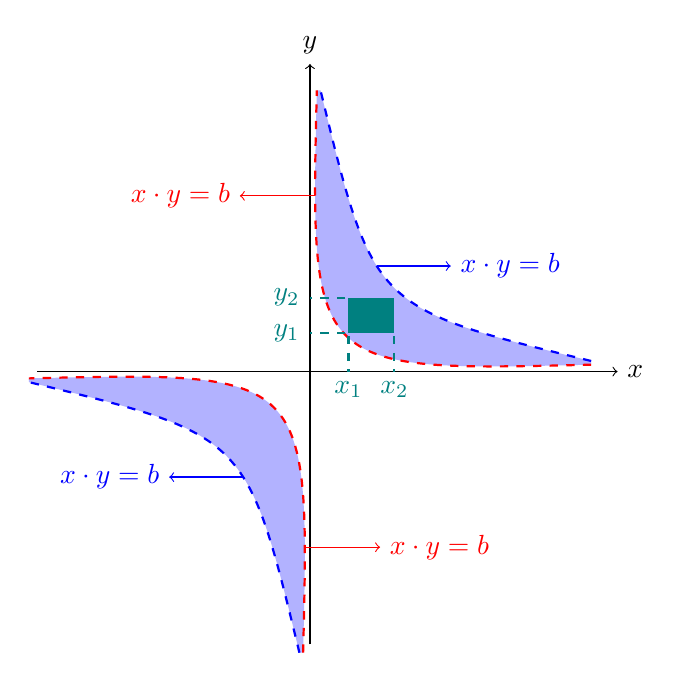
\begin{tikzpicture}[scale=0.67] % Scale everything to 2/3
    
        % Define parameters
        \def\a{1.33}  % Scaled to 2/3
        \def\b{3.33}  % Scaled to 2/3
        \def\xmin{-2.67}  % Scaled to 2/3
        \def\xmax{3.33}  % Scaled to 2/3
        \def\ymin{-2.67}  % Scaled to 2/3
        \def\ymax{3.33}  % Scaled to 2/3

        \fill[blue!30] 
        (\xmax+2, 0.13) .. controls (0,0) .. (0.13, \ymax+2)
        -- 
        (0.2, \ymax+2) .. controls (1.2,1.2) .. (\xmax+2, 0.2)
        -- cycle;

        % negative part
        \fill[blue!30] 
        (-0.13, -\xmax-2) .. controls (0,0) .. (-\ymax-2, -0.13)
        -- 
        (-\ymax-2, -0.2) .. controls (-1.2,-1.2) .. (-0.2, -\xmax-2)
        -- cycle;

        % positive part
        \draw[thick, red, dashed] (\xmax+2, 0.13) ..controls (0,0) .. (0.13, \ymax+2);
        \draw[thick, blue, dashed] (\xmax+2, 0.2) ..controls (1.2,1.2) .. (0.2, \ymax+2);
        
        % Reflected lines
        \draw[thick, red, dashed] (-0.13, -\xmax-2) .. controls (0,0) .. (-\ymax-2, -0.13);
        \draw[thick, blue, dashed] (-0.2, -\xmax-2) .. controls (-1.2,-1.2) .. (-\ymax-2, -0.2);

        % Axes
        \draw[->] (\xmin-2.5, 0) -- (\xmax+2.5, 0) node[right] {$x$};
        \draw[->] (0, \ymin-2.5) -- (0, \ymax+2.5) node[above] {$y$};

        % square
        \fill[teal] (0.73, 0.73) rectangle (1.6, 1.4);

        % labels
        \draw[thick, teal, dashed] (0.67,0.73) -- (0,0.73) node[left] {$y_1$};
        \draw[thick, teal, dashed] (1.6,0.67) -- (1.6,0) node[below] {$x_2$};
        \draw[thick, teal, dashed] (0.67,1.4) -- (0,1.4) node[left] {$y_2$};
        \draw[thick, teal, dashed] (0.73,0.67) -- (0.73,0) node[below] {$x_1$};

        % labels
        \draw[blue, ->] (1.27, 2) -- (2.67, 2) node[right] {$x \cdot y = b$};
        \draw[blue, ->] (-1.27, -2) -- (-2.67, -2) node[left] {$x \cdot y = b$};
        \draw[red, ->] (0.1, 3.33) -- (-1.33, 3.33) node[left] {$x \cdot y = b$};
        \draw[red, ->] (-0.1, -3.33) -- (1.33, -3.33) node[right] {$x \cdot y = b$};
        
    \end{tikzpicture}
\end{figure}


\end{proof}
\begin{theorem}[Multiplication]
\label{thm::multiplication_has_OEX}
     Let $f,g:\Reals\to \Reals$ be \effectivelyOpen. Then $(f\cdot g)$ is also \effectivelyOpen.
\end{theorem}
\begin{proof}
       Using Theorem \ref{thm::composition_has_OEX}, we know that compositions preserve \effectivelyOpen\text{ness}. Now we know that $(f\cdot g)$ is composed from the functions $\CartProd$, $\Diag$, and $\Mult$. Therefore Lemmas \ref{claim::cartprod-effectively-open}, \ref{claim::diag-effectively-open}, and \ref{claim::mult-effectively-open} complete the proof.
\end{proof}